\documentclass[twoside]{book}

% Packages required by doxygen
\usepackage{fixltx2e}
\usepackage{calc}
\usepackage{doxygen}
\usepackage[export]{adjustbox} % also loads graphicx
\usepackage{graphicx}
\usepackage[utf8]{inputenc}
\usepackage{makeidx}
\usepackage{multicol}
\usepackage{multirow}
\PassOptionsToPackage{warn}{textcomp}
\usepackage{textcomp}
\usepackage[nointegrals]{wasysym}
\usepackage[table]{xcolor}

% Font selection
\usepackage[T1]{fontenc}
\usepackage[scaled=.90]{helvet}
\usepackage{courier}
\usepackage{amssymb}
\usepackage{sectsty}
\renewcommand{\familydefault}{\sfdefault}
\allsectionsfont{%
  \fontseries{bc}\selectfont%
  \color{darkgray}%
}
\renewcommand{\DoxyLabelFont}{%
  \fontseries{bc}\selectfont%
  \color{darkgray}%
}
\newcommand{\+}{\discretionary{\mbox{\scriptsize$\hookleftarrow$}}{}{}}

% Page & text layout
\usepackage{geometry}
\geometry{%
  a4paper,%
  top=2.5cm,%
  bottom=2.5cm,%
  left=2.5cm,%
  right=2.5cm%
}
\tolerance=750
\hfuzz=15pt
\hbadness=750
\setlength{\emergencystretch}{15pt}
\setlength{\parindent}{0cm}
\setlength{\parskip}{0.2cm}
\makeatletter
\renewcommand{\paragraph}{%
  \@startsection{paragraph}{4}{0ex}{-1.0ex}{1.0ex}{%
    \normalfont\normalsize\bfseries\SS@parafont%
  }%
}
\renewcommand{\subparagraph}{%
  \@startsection{subparagraph}{5}{0ex}{-1.0ex}{1.0ex}{%
    \normalfont\normalsize\bfseries\SS@subparafont%
  }%
}
\makeatother

% Headers & footers
\usepackage{fancyhdr}
\pagestyle{fancyplain}
\fancyhead[LE]{\fancyplain{}{\bfseries\thepage}}
\fancyhead[CE]{\fancyplain{}{}}
\fancyhead[RE]{\fancyplain{}{\bfseries\leftmark}}
\fancyhead[LO]{\fancyplain{}{\bfseries\rightmark}}
\fancyhead[CO]{\fancyplain{}{}}
\fancyhead[RO]{\fancyplain{}{\bfseries\thepage}}
\fancyfoot[LE]{\fancyplain{}{}}
\fancyfoot[CE]{\fancyplain{}{}}
\fancyfoot[RE]{\fancyplain{}{\bfseries\scriptsize Generated on Tue Mar 29 2016 22\+:47\+:17 for Practica 3 by Doxygen }}
\fancyfoot[LO]{\fancyplain{}{\bfseries\scriptsize Generated on Tue Mar 29 2016 22\+:47\+:17 for Practica 3 by Doxygen }}
\fancyfoot[CO]{\fancyplain{}{}}
\fancyfoot[RO]{\fancyplain{}{}}
\renewcommand{\footrulewidth}{0.4pt}
\renewcommand{\chaptermark}[1]{%
  \markboth{#1}{}%
}
\renewcommand{\sectionmark}[1]{%
  \markright{\thesection\ #1}%
}

% Indices & bibliography
\usepackage{natbib}
\usepackage[titles]{tocloft}
\setcounter{tocdepth}{3}
\setcounter{secnumdepth}{5}
\makeindex

% Hyperlinks (required, but should be loaded last)
\usepackage{ifpdf}
\ifpdf
  \usepackage[pdftex,pagebackref=true]{hyperref}
\else
  \usepackage[ps2pdf,pagebackref=true]{hyperref}
\fi
\hypersetup{%
  colorlinks=true,%
  linkcolor=blue,%
  citecolor=blue,%
  unicode%
}

% Custom commands
\newcommand{\clearemptydoublepage}{%
  \newpage{\pagestyle{empty}\cleardoublepage}%
}


%===== C O N T E N T S =====

\begin{document}

% Titlepage & ToC
\hypersetup{pageanchor=false,
             bookmarks=true,
             bookmarksnumbered=true,
             pdfencoding=unicode
            }
\pagenumbering{roman}
\begin{titlepage}
\vspace*{7cm}
\begin{center}%
{\Large Practica 3 }\\
\vspace*{1cm}
{\large Generated by Doxygen 1.8.9.1}\\
\vspace*{0.5cm}
{\small Tue Mar 29 2016 22:47:17}\\
\end{center}
\end{titlepage}
\clearemptydoublepage
\tableofcontents
\clearemptydoublepage
\pagenumbering{arabic}
\hypersetup{pageanchor=true}

%--- Begin generated contents ---
\chapter{Hierarchical Index}
\section{Class Hierarchy}
This inheritance list is sorted roughly, but not completely, alphabetically\+:\begin{DoxyCompactList}
\item \contentsline{section}{Practica4.\+Arbitro}{\pageref{class_practica4_1_1_arbitro}}{}
\item \contentsline{section}{Practica4.\+Pelota}{\pageref{class_practica4_1_1_pelota}}{}
\item Runnable\begin{DoxyCompactList}
\item \contentsline{section}{Practica4.\+Jugador}{\pageref{class_practica4_1_1_jugador}}{}
\end{DoxyCompactList}
\end{DoxyCompactList}

\chapter{Class Index}
\section{Lista de clases}
Lista de las clases, estructuras, uniones e interfaces con una breve descripción\+:\begin{DoxyCompactList}
\item\contentsline{section}{\hyperlink{class_ejercicio1__3__3_1_1_detener___interrupcion}{Ejercicio1\+\_\+3\+\_\+3.\+Detener\+\_\+\+Interrupcion} \\*Thread que se detiene tras una señal del usuario, con diferentes acciones en función del tiempo transcurrido }{\pageref{class_ejercicio1__3__3_1_1_detener___interrupcion}}{}
\item\contentsline{section}{\hyperlink{class_ejercicio1__2__1_1_1_ejercicio1}{Ejercicio1\+\_\+2\+\_\+1.\+Ejercicio1} \\*Creación del número de hilos especificados por el usuario }{\pageref{class_ejercicio1__2__1_1_1_ejercicio1}}{}
\item\contentsline{section}{\hyperlink{class_ejercicio1__2__1_1_1_ejercicio2}{Ejercicio1\+\_\+2\+\_\+1.\+Ejercicio2} \\*Creación del número de hilos especificados por el usuario y medición del tiempo de ejecucion de los hilos }{\pageref{class_ejercicio1__2__1_1_1_ejercicio2}}{}
\item\contentsline{section}{\hyperlink{class_ejercicio1__2__4_1_1_ejercicio4}{Ejercicio1\+\_\+2\+\_\+4.\+Ejercicio4} \\*Cada thread calcula su tiempo de ejecución, lo almacena en una variable publica y se calcula el tiempo total }{\pageref{class_ejercicio1__2__4_1_1_ejercicio4}}{}
\item\contentsline{section}{\hyperlink{class_ejercicio1__2__5_1_1_ejercicio5}{Ejercicio1\+\_\+2\+\_\+5.\+Ejercicio5} \\*Muestra por separados los tiempos de inicialización de threads y los tiempos de ejecución de threads }{\pageref{class_ejercicio1__2__5_1_1_ejercicio5}}{}
\item\contentsline{section}{\hyperlink{class_ejercicio1__2__6_1_1_ejercicio6}{Ejercicio1\+\_\+2\+\_\+6.\+Ejercicio6} \\*Al crear los threads, en caso de introducir el valor \char`\"{}1\char`\"{} se realiza una operación compleja, en caso contrario se procede a la identificación finalización de los threads }{\pageref{class_ejercicio1__2__6_1_1_ejercicio6}}{}
\item\contentsline{section}{\hyperlink{class_ejercicio1__1__2_1_1hello_runnable}{Ejercicio1\+\_\+1\+\_\+2.\+hello\+Runnable} \\*Creación de hilos usando la clase Runnable }{\pageref{class_ejercicio1__1__2_1_1hello_runnable}}{}
\item\contentsline{section}{\hyperlink{class_ejercicio1__1__3_1_1hello_runnable___sleep}{Ejercicio1\+\_\+1\+\_\+3.\+hello\+Runnable\+\_\+\+Sleep} \\*Creación de hilos usando la clase Runnable y usando el método sleep para crear el delay de 1 segundo }{\pageref{class_ejercicio1__1__3_1_1hello_runnable___sleep}}{}
\item\contentsline{section}{\hyperlink{class_ejercicio1__1__2_1_1hello_thread}{Ejercicio1\+\_\+1\+\_\+2.\+hello\+Thread} \\*Creación de hilos usando la clase Thread }{\pageref{class_ejercicio1__1__2_1_1hello_thread}}{}
\item\contentsline{section}{\hyperlink{class_ejercicio1__1__3_1_1hello_thread___sleep}{Ejercicio1\+\_\+1\+\_\+3.\+hello\+Thread\+\_\+\+Sleep} \\*Creación de hilos usando la clase Thread y usando el método sleep para crear el delay de 1 segundo }{\pageref{class_ejercicio1__1__3_1_1hello_thread___sleep}}{}
\item\contentsline{section}{\hyperlink{class_ejercicio1__1__4_1_1_runnable___activo}{Ejercicio1\+\_\+1\+\_\+4.\+Runnable\+\_\+\+Activo} \\*Creación de hilos usando la clase Runnable y usando los metodos active\+Count y current\+Thread para postrar el numero de hilos y el hilo actual }{\pageref{class_ejercicio1__1__4_1_1_runnable___activo}}{}
\item\contentsline{section}{\hyperlink{class_ejercicio1__1__4_1_1_thread___activo}{Ejercicio1\+\_\+1\+\_\+4.\+Thread\+\_\+\+Activo} \\*Creación de hilos usando la clase Thread y usando los metodos active\+Count y current\+Thread para postrar el numero de hilos y el hilo actual }{\pageref{class_ejercicio1__1__4_1_1_thread___activo}}{}
\item\contentsline{section}{\hyperlink{class_ejercicio1__3__2_1_1_thread___detenido}{Ejercicio1\+\_\+3\+\_\+2.\+Thread\+\_\+\+Detenido} \\*Crea un Thread y comprueba con is\+Interrupted() e interrupted() antes y después de interrumpirlo }{\pageref{class_ejercicio1__3__2_1_1_thread___detenido}}{}
\end{DoxyCompactList}

\chapter{Class Documentation}
\hypertarget{class_practica3_1_1_a}{}\section{Practica3.\+A Class Reference}
\label{class_practica3_1_1_a}\index{Practica3.\+A@{Practica3.\+A}}


Clase encargada de mostrar la ejecución del hilo.  


\subsection*{Public Member Functions}
\begin{DoxyCompactItemize}
\item 
void \hyperlink{class_practica3_1_1_a_aba405116e569ea00ef5800906f331cd8}{Enter\+And\+Wait} ()
\begin{DoxyCompactList}\small\item\em Método que implementa un delay de 3 segundos. \end{DoxyCompactList}\end{DoxyCompactItemize}


\subsection{Detailed Description}
Clase encargada de mostrar la ejecución del hilo. 

\begin{DoxyAuthor}{Author}
Nara, Javier, Esteban 
\end{DoxyAuthor}


\subsection{Member Function Documentation}
\hypertarget{class_practica3_1_1_a_aba405116e569ea00ef5800906f331cd8}{}\index{Practica3\+::\+A@{Practica3\+::\+A}!Enter\+And\+Wait@{Enter\+And\+Wait}}
\index{Enter\+And\+Wait@{Enter\+And\+Wait}!Practica3\+::\+A@{Practica3\+::\+A}}
\subsubsection[{Enter\+And\+Wait}]{\setlength{\rightskip}{0pt plus 5cm}void Practica3.\+A.\+Enter\+And\+Wait (
\begin{DoxyParamCaption}
{}
\end{DoxyParamCaption}
)}\label{class_practica3_1_1_a_aba405116e569ea00ef5800906f331cd8}


Método que implementa un delay de 3 segundos. 

\begin{DoxyAuthor}{Author}
Nara, Javier, Esteban 
\end{DoxyAuthor}


The documentation for this class was generated from the following file\+:\begin{DoxyCompactItemize}
\item 
A.\+java\end{DoxyCompactItemize}

\hypertarget{class_practica3_1_1_b}{}\section{Practica3.\+B Class Reference}
\label{class_practica3_1_1_b}\index{Practica3.\+B@{Practica3.\+B}}


Clase que implementa runnable y contiene un valor de tipo \hyperlink{class_practica3_1_1_a}{A} para su ejecución mediante hilos.  




Inheritance diagram for Practica3.\+B\+:
\nopagebreak
\begin{figure}[H]
\begin{center}
\leavevmode
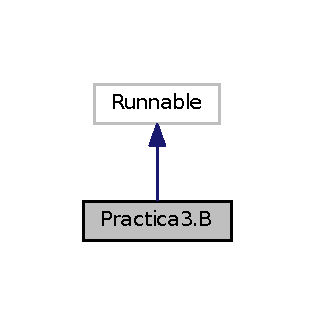
\includegraphics[width=151pt]{class_practica3_1_1_b__inherit__graph}
\end{center}
\end{figure}


Collaboration diagram for Practica3.\+B\+:
\nopagebreak
\begin{figure}[H]
\begin{center}
\leavevmode
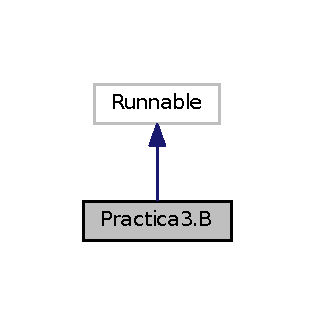
\includegraphics[width=151pt]{class_practica3_1_1_b__coll__graph}
\end{center}
\end{figure}
\subsection*{Public Member Functions}
\begin{DoxyCompactItemize}
\item 
\hypertarget{class_practica3_1_1_b_a23ae5af09f37cb24c03cf152e07d5448}{}{\bfseries B} (\hyperlink{class_practica3_1_1_a}{A} valor\+A)\label{class_practica3_1_1_b_a23ae5af09f37cb24c03cf152e07d5448}

\item 
void \hyperlink{class_practica3_1_1_b_afd28d42d2ac7d35ac97c3969f82bf9f5}{run} ()
\begin{DoxyCompactList}\small\item\em Método run que implementa los threads. \end{DoxyCompactList}\end{DoxyCompactItemize}


\subsection{Detailed Description}
Clase que implementa runnable y contiene un valor de tipo \hyperlink{class_practica3_1_1_a}{A} para su ejecución mediante hilos. 

\begin{DoxyAuthor}{Author}
Nara, Javier, Esteban 
\end{DoxyAuthor}


\subsection{Member Function Documentation}
\hypertarget{class_practica3_1_1_b_afd28d42d2ac7d35ac97c3969f82bf9f5}{}\index{Practica3\+::\+B@{Practica3\+::\+B}!run@{run}}
\index{run@{run}!Practica3\+::\+B@{Practica3\+::\+B}}
\subsubsection[{run}]{\setlength{\rightskip}{0pt plus 5cm}void Practica3.\+B.\+run (
\begin{DoxyParamCaption}
{}
\end{DoxyParamCaption}
)}\label{class_practica3_1_1_b_afd28d42d2ac7d35ac97c3969f82bf9f5}


Método run que implementa los threads. 

\begin{DoxyAuthor}{Author}
Nara, Javier, Esteban 
\end{DoxyAuthor}


The documentation for this class was generated from the following file\+:\begin{DoxyCompactItemize}
\item 
B.\+java\end{DoxyCompactItemize}

\hypertarget{class_practica3_1_1_contador}{}\section{Practica3.\+Contador Class Reference}
\label{class_practica3_1_1_contador}\index{Practica3.\+Contador@{Practica3.\+Contador}}


Clase que realiza el incremento de una variable.  


\subsection*{Public Member Functions}
\begin{DoxyCompactItemize}
\item 
int \hyperlink{class_practica3_1_1_contador_afb21d477bad87ddf134288d34842ba81}{incrementar} (int n)
\begin{DoxyCompactList}\small\item\em Método que realiza el incremento de la variable valor. \end{DoxyCompactList}\end{DoxyCompactItemize}


\subsection{Detailed Description}
Clase que realiza el incremento de una variable. 

\begin{DoxyAuthor}{Author}
Nara, Javier, Esteban 
\end{DoxyAuthor}


\subsection{Member Function Documentation}
\hypertarget{class_practica3_1_1_contador_afb21d477bad87ddf134288d34842ba81}{}\index{Practica3\+::\+Contador@{Practica3\+::\+Contador}!incrementar@{incrementar}}
\index{incrementar@{incrementar}!Practica3\+::\+Contador@{Practica3\+::\+Contador}}
\subsubsection[{incrementar}]{\setlength{\rightskip}{0pt plus 5cm}int Practica3.\+Contador.\+incrementar (
\begin{DoxyParamCaption}
\item[{int}]{n}
\end{DoxyParamCaption}
)}\label{class_practica3_1_1_contador_afb21d477bad87ddf134288d34842ba81}


Método que realiza el incremento de la variable valor. 

\begin{DoxyAuthor}{Author}
Nara, Javier, Esteban  int n \+: Número de incrementos a realizar 
\end{DoxyAuthor}
\begin{DoxyReturn}{Returns}
valor \+: Valor de la variable luego de realizar todos los incrementos 
\end{DoxyReturn}


The documentation for this class was generated from the following file\+:\begin{DoxyCompactItemize}
\item 
Contador.\+java\end{DoxyCompactItemize}

\hypertarget{class_practica3_1_1_control}{}\section{Practica3.\+Control Class Reference}
\label{class_practica3_1_1_control}\index{Practica3.\+Control@{Practica3.\+Control}}


Clase que implementa el main y se encarga de realizar la ejecución de threads con objetos de la clase \hyperlink{class_practica3_1_1_b}{B} y en la cuál solo un thread puede ejecutar el método enter Enter\+And\+Wait()  


\subsection*{Static Public Member Functions}
\begin{DoxyCompactItemize}
\item 
\hypertarget{class_practica3_1_1_control_a902225128c6668c45c8b5eacd0ab21c5}{}static void {\bfseries main} (String\mbox{[}$\,$\mbox{]} args)  throws Interrupted\+Exception\label{class_practica3_1_1_control_a902225128c6668c45c8b5eacd0ab21c5}

\end{DoxyCompactItemize}


\subsection{Detailed Description}
Clase que implementa el main y se encarga de realizar la ejecución de threads con objetos de la clase \hyperlink{class_practica3_1_1_b}{B} y en la cuál solo un thread puede ejecutar el método enter Enter\+And\+Wait() 

\begin{DoxyAuthor}{Author}
Nara, Javier, Esteban 
\end{DoxyAuthor}


The documentation for this class was generated from the following file\+:\begin{DoxyCompactItemize}
\item 
Control.\+java\end{DoxyCompactItemize}

\hypertarget{class_practica3_1_1_control1}{}\section{Practica3.\+Control1 Class Reference}
\label{class_practica3_1_1_control1}\index{Practica3.\+Control1@{Practica3.\+Control1}}


Clase que implementa el main y se encarga de realizar la ejecución de threads con objetos de la clase \hyperlink{class_practica3_1_1_b}{B} y en la cuál todos los threads pueden ejecutar el método enter Enter\+And\+Wait()  


\subsection*{Static Public Member Functions}
\begin{DoxyCompactItemize}
\item 
\hypertarget{class_practica3_1_1_control1_a58e402b0152caaf34e119ab278ddeb71}{}static void {\bfseries main} (String\mbox{[}$\,$\mbox{]} args)\label{class_practica3_1_1_control1_a58e402b0152caaf34e119ab278ddeb71}

\end{DoxyCompactItemize}


\subsection{Detailed Description}
Clase que implementa el main y se encarga de realizar la ejecución de threads con objetos de la clase \hyperlink{class_practica3_1_1_b}{B} y en la cuál todos los threads pueden ejecutar el método enter Enter\+And\+Wait() 

\begin{DoxyAuthor}{Author}
Nara, Javier, Esteban 
\end{DoxyAuthor}


The documentation for this class was generated from the following file\+:\begin{DoxyCompactItemize}
\item 
Control1.\+java\end{DoxyCompactItemize}

\hypertarget{class_practica3_1_1_hilo}{}\section{Practica3.\+Hilo Class Reference}
\label{class_practica3_1_1_hilo}\index{Practica3.\+Hilo@{Practica3.\+Hilo}}


Clase que implementa el main, además incluye la ejecución de threads.  




Inheritance diagram for Practica3.\+Hilo\+:
\nopagebreak
\begin{figure}[H]
\begin{center}
\leavevmode
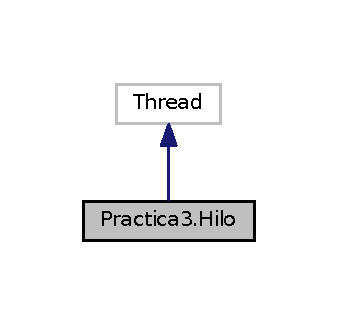
\includegraphics[width=162pt]{class_practica3_1_1_hilo__inherit__graph}
\end{center}
\end{figure}


Collaboration diagram for Practica3.\+Hilo\+:
\nopagebreak
\begin{figure}[H]
\begin{center}
\leavevmode
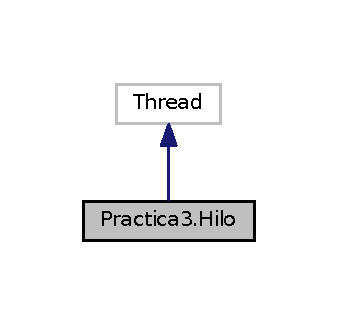
\includegraphics[width=162pt]{class_practica3_1_1_hilo__coll__graph}
\end{center}
\end{figure}
\subsection*{Public Member Functions}
\begin{DoxyCompactItemize}
\item 
\hyperlink{class_practica3_1_1_hilo_a6b92ae49828258f59927af9eebbdc81d}{Hilo} (int n, int incremento, \hyperlink{class_practica3_1_1_contador}{Contador} contador)
\begin{DoxyCompactList}\small\item\em Método constructor de la clase. \end{DoxyCompactList}\item 
void \hyperlink{class_practica3_1_1_hilo_ae8e47d60f2c0045078cf1dbcab6c5a1f}{run} ()
\begin{DoxyCompactList}\small\item\em Método que implementa la ejecución de los threads. \end{DoxyCompactList}\end{DoxyCompactItemize}
\subsection*{Static Public Member Functions}
\begin{DoxyCompactItemize}
\item 
static void \hyperlink{class_practica3_1_1_hilo_af75a2ba35b3a63c2d3525d923926641c}{main} (String\mbox{[}$\,$\mbox{]} args)
\end{DoxyCompactItemize}


\subsection{Detailed Description}
Clase que implementa el main, además incluye la ejecución de threads. 

\begin{DoxyAuthor}{Author}
Nara, Javier, Esteban 
\end{DoxyAuthor}


\subsection{Constructor \& Destructor Documentation}
\hypertarget{class_practica3_1_1_hilo_a6b92ae49828258f59927af9eebbdc81d}{}\index{Practica3\+::\+Hilo@{Practica3\+::\+Hilo}!Hilo@{Hilo}}
\index{Hilo@{Hilo}!Practica3\+::\+Hilo@{Practica3\+::\+Hilo}}
\subsubsection[{Hilo}]{\setlength{\rightskip}{0pt plus 5cm}Practica3.\+Hilo.\+Hilo (
\begin{DoxyParamCaption}
\item[{int}]{n, }
\item[{int}]{incremento, }
\item[{{\bf Contador}}]{contador}
\end{DoxyParamCaption}
)}\label{class_practica3_1_1_hilo_a6b92ae49828258f59927af9eebbdc81d}


Método constructor de la clase. 

\begin{DoxyAuthor}{Author}
Nara, Javier, Esteban \begin{DoxyItemize}
\item int n \+: Número de thread \item int incremento \+: Número de veces que se realizará el incremento \item \hyperlink{class_practica3_1_1_contador}{Contador} contador \+: \hyperlink{class_practica3_1_1_contador}{Contador} creado \end{DoxyItemize}

\end{DoxyAuthor}


\subsection{Member Function Documentation}
\hypertarget{class_practica3_1_1_hilo_af75a2ba35b3a63c2d3525d923926641c}{}\index{Practica3\+::\+Hilo@{Practica3\+::\+Hilo}!main@{main}}
\index{main@{main}!Practica3\+::\+Hilo@{Practica3\+::\+Hilo}}
\subsubsection[{main}]{\setlength{\rightskip}{0pt plus 5cm}static void Practica3.\+Hilo.\+main (
\begin{DoxyParamCaption}
\item[{String\mbox{[}$\,$\mbox{]}}]{args}
\end{DoxyParamCaption}
)\hspace{0.3cm}{\ttfamily [static]}}\label{class_practica3_1_1_hilo_af75a2ba35b3a63c2d3525d923926641c}

\begin{DoxyParams}{Parameters}
{\em args} & \\
\hline
\end{DoxyParams}
\hypertarget{class_practica3_1_1_hilo_ae8e47d60f2c0045078cf1dbcab6c5a1f}{}\index{Practica3\+::\+Hilo@{Practica3\+::\+Hilo}!run@{run}}
\index{run@{run}!Practica3\+::\+Hilo@{Practica3\+::\+Hilo}}
\subsubsection[{run}]{\setlength{\rightskip}{0pt plus 5cm}void Practica3.\+Hilo.\+run (
\begin{DoxyParamCaption}
{}
\end{DoxyParamCaption}
)}\label{class_practica3_1_1_hilo_ae8e47d60f2c0045078cf1dbcab6c5a1f}


Método que implementa la ejecución de los threads. 

\begin{DoxyAuthor}{Author}
Nara, Javier, Esteban 
\end{DoxyAuthor}


The documentation for this class was generated from the following file\+:\begin{DoxyCompactItemize}
\item 
Hilo.\+java\end{DoxyCompactItemize}

%--- End generated contents ---

% Index
\backmatter
\newpage
\phantomsection
\clearemptydoublepage
\addcontentsline{toc}{chapter}{Index}
\printindex

\end{document}
